\documentclass[12pt]{article}
\usepackage{import}
%===============================%
%  Packages and basic settings  %
%===============================%
\usepackage[letterpaper, left=1.25in, right=1.25in, top=1in, bottom=1in]{geometry}
\usepackage{amssymb}
\usepackage{amsmath}
\usepackage{enumitem}
\usepackage{hyperref}
\usepackage[hyperref,amsthm,amsmath,framed,thmmarks]{ntheorem}
\usepackage[capitalise,noabbrev]{cleveref}
\usepackage{tikz}
\usepackage{tikz-cd}
\usetikzlibrary{braids,arrows,decorations.markings,calc}

%====================================%
%  Theorems, environments & cleveref  %
%====================================%
\theoremstyle{plain}
\newtheorem{theorem}{Theorem}[section]
\newtheorem{proposition}[theorem]{Proposition}
\newtheorem{corollary}[theorem]{Corollary}
\newtheorem{lemma}[theorem]{Lemma}

\theoremstyle{nonumberplain}
\renewtheorem{theorem*}{Theorem}
\renewtheorem{proposition*}{Proposition}
\renewtheorem{corollary*}{Corollary}
\renewtheorem{lemma*}{Lemma}

\theoremstyle{remark}
\newtheorem{conjecture}[theorem]{Conjecture}
\newtheorem{remark}[theorem]{Remark}
\newtheorem{problem}[theorem]{Open Problem}
\newtheorem{heuristic}[theorem]{Heuristic}

\theoremstyle{nonumberplain}
\renewtheorem{conjecture*}{Conjecture}
\renewtheorem{remark*}{Remark}
\renewtheorem{problem*}{Open Problem}
\renewtheorem{heuristic*}{Heuristic}

%==================================%
%  Custom commands & environments  %
%==================================%
\newcommand{\legendre}[2]{\left(\frac{#1}{#2}\right)}
\newcommand{\dlegendre}[2]{\displaystyle{\left(\frac{#1}{#2}\right)}}
\newcommand{\tlegendre}[2]{\textstyle{\left(\frac{#1}{#2}\right)}}
\newcommand{\psum}{\sideset{}{'}\sum}
\newcommand{\asum}{\sideset{}{^{\ast}}\sum}
\newcommand{\tmod}[1]{\ (\mathrm{mod}\text{ }#1)}
\renewcommand{\bmod}[1]{\ \left(\mathrm{mod}\text{ }#1\right)}
\newcommand{\xto}[1]{\xrightarrow{#1}}
\newcommand{\xfrom}[1]{\xleftarrow{#1}}
\newcommand{\normal}{\mathrel{\unlhd}}
\newcommand{\mf}{\mathfrak}
\newcommand{\mc}{\mathcal}
\newcommand{\ms}{\mathscr}

\newcommand{\Mat}{\mathrm{Mat}}
\newcommand{\GL}{\mathrm{GL}}
\newcommand{\SL}{\mathrm{SL}}
\newcommand{\PSL}{\mathrm{PSL}}
\renewcommand{\O}{\mathrm{O}}
\newcommand{\SO}{\mathrm{SO}}
\newcommand{\U}{\mathrm{U}}
\newcommand{\Sp}{\mathrm{Sp}}

\newcommand{\N}{\mathbb{N}}
\newcommand{\Z}{\mathbb{Z}}
\newcommand{\Q}{\mathbb{Q}}
\newcommand{\R}{\mathbb{R}}
\newcommand{\C}{\mathbb{C}}
\newcommand{\F}{\mathbb{F}}
\renewcommand{\H}{\mathbb{H}}
\renewcommand{\P}{\mathbb{P}}

\renewcommand{\a}{\alpha}
\renewcommand{\b}{\beta}
\newcommand{\g}{\gamma}
\renewcommand{\d}{\delta}
\newcommand{\z}{\zeta}
\renewcommand{\t}{\theta}
\renewcommand{\i}{\iota}
\renewcommand{\k}{\kappa}
\renewcommand{\l}{\lambda}
\newcommand{\s}{\sigma}
\newcommand{\w}{\omega}

\newcommand{\G}{\Gamma}
\newcommand{\D}{\Delta}
\renewcommand{\L}{\Lambda}
\newcommand{\W}{\Omega}
\newcommand{\scL}{\mathscr{L}}

\newcommand{\e}{\varepsilon}
\newcommand{\vt}{\vartheta}
\newcommand{\vphi}{\varphi}
\newcommand{\emt}{\varnothing}

\newcommand{\x}{\times}
\newcommand{\ox}{\otimes}
\newcommand{\op}{\oplus}
\newcommand{\bigox}{\bigotimes}
\newcommand{\bigop}{\bigoplus}
\newcommand{\del}{\partial}
\newcommand{\<}{\langle}
\renewcommand{\>}{\rangle}
\newcommand{\lf}{\lfloor}
\newcommand{\rf}{\rfloor}
\newcommand{\wtilde}{\widetilde}
\newcommand{\what}{\widehat}
\newcommand{\conj}{\overline}
\newcommand{\cchi}{\conj{\chi}}

\DeclareMathOperator{\id}{\textrm{id}}
\DeclareMathOperator{\sgn}{\mathrm{sgn}}
\DeclareMathOperator{\im}{\mathrm{im}}
\DeclareMathOperator{\rk}{\mathrm{rk}}
\DeclareMathOperator{\adj}{\mathrm{adj}}
\DeclareMathOperator{\tr}{\mathrm{trace}}
\DeclareMathOperator{\nm}{\mathrm{norm}}
\DeclareMathOperator{\disc}{\mathrm{disc}}
\DeclareMathOperator{\ord}{\mathrm{ord}}
\DeclareMathOperator{\sym}{\mathrm{sym}}
\DeclareMathOperator{\ext}{\mathrm{ext}}
\DeclareMathOperator{\Hom}{\mathrm{Hom}}
\DeclareMathOperator{\End}{\mathrm{End}}
\DeclareMathOperator{\Aut}{\mathrm{Aut}}
\DeclareMathOperator{\Tor}{\mathrm{Tor}}
\DeclareMathOperator{\Ann}{\mathrm{Ann}}
\DeclareMathOperator{\Gal}{\mathrm{Gal}}
\DeclareMathOperator{\Trace}{\mathrm{Tr}}
\DeclareMathOperator{\Norm}{\mathrm{N}}
\DeclareMathOperator{\Cl}{\mathrm{Cl}}
\DeclareMathOperator{\Span}{\mathrm{Span}}
\DeclareMathOperator*{\Res}{\mathrm{Res}}
\DeclareMathOperator{\Vol}{\mathrm{Vol}}
\DeclareMathOperator{\Li}{\mathrm{Li}}
\DeclareMathOperator{\Supp}{\mathrm{Supp}}
\renewcommand{\Re}{\mathrm{Re}}
\renewcommand{\Im}{\mathrm{Im}}
\DeclareMathOperator{\Ph}{\mathrm{Ph}}
\DeclareMathOperator{\SC}{\mathrm{SC}}


\newcommand{\GH}{\G\backslash\H}
\newcommand{\GG}{\G_{\infty}\backslash\G}

\newenvironment{psmallmatrix}
  {\left(\begin{smallmatrix}}
  {\end{smallmatrix}\right)}

\newcommand{\smc}[1]{
    \mathchoice
    {{\scriptstyle\mathcal{#1}}}
    {{\scriptstyle\mathcal{#1}}}
    {{\scriptscriptstyle\mathcal{#1}}}
    {\scalebox{0.7}{$\scriptscriptstyle\mathcal{#1}$}}
}

%============%
%  Comments  %
%============%
\newcommand{\todo}[1]{\textcolor{red}{\sf Todo: [#1]}}

%===================%
%  Label reminders  %
%===================%
% [label=(\roman*)]
% [label=(\alph*)]
% [label=(\arabic{enumi})]

%==================%
%  Other settings  %
%==================%
\pgfdeclarelayer{background}
\pgfsetlayers{background,main}
\tikzset{->-/.style={decoration={
  markings,
  mark=at position .5 with {\arrow{>}}},postaction={decorate}}}

%=================%
%  Title & Index  %
%=================%
\title{The Gamma function}
\author{Henry Twiss}
\makeindex

\begin{document}
  \date{}
  \maketitle
  Throughout, \(s = \s+it\) and \(u = \tau+ir\) will stand for complex variables with \(\s\), \(\tau\), \(t\), and \(r\) real. 
  \section{Analytic Properties}
    The \textit{gamma function} \(\G(s)\) is defined by the integral
    \[
      \G(s) = \int_{0}^{\infty}e^{-x}x^{s-1}\,dx.
    \]
    Equivalently, \(\G(s)\) is the Mellin transform of \(e^{-x}\). This defines a holomorphic function for \(\s > 0\). Indeed, writing
    \[
      \G(s) = \int_{0}^{1}e^{-x}x^{s-1}\,dx+\int_{1}^{\infty}e^{-x}x^{s-1}\,dx,
    \]
    both integrals are locally absolutely uniformly convergent in this half-plane. Also note that \(\G(s)\) is real for \(s > 0\). The most basic properties of \(\G(s)\) are collected in the following result:

    \begin{proposition}\label{prop:Factorial_properties_of_gamma_function}
      \(\G(s)\) satisfies
      \[
         \G(1) = 1 \quad \text{and} \quad \G(s+1) = s\G(s).
      \]
      In particular,
      \[
        \G(n) = (n-1)!,
      \]
      for any positive integer \(n\). Also,
      \[
        \G(\conj{s}) = \conj{\G(s)}.
      \]
    \end{proposition}
    \begin{proof}
      The first identity follow by direct evaluation. The second is a direct computation requiring an application of integration by parts. The following statement is obtained by repeated application of the latter identity. The last statement follows from the identity theorem and that \(\G(s)\) is real for \(\s > 1\).
    \end{proof}

    In light of \(\G(n) = (n-1)!\), we can view \(\G(s)\) as a holomorphic extension of the factorial function. An interesting observation is the value that this extension takes at \(s = \frac{1}{2}\). The change of variables \(x \mapsto \pi x^{2}\) transforms the integral defining \(\G\left(\frac{1}{2}\right)\) into a Gaussian integral giving
    \begin{equation}\label{equ:gamma_function_at_1/2}
      \G\left(\frac{1}{2}\right) = \pi\int_{-\infty}^{\infty}e^{-\pi x^{2}}\,dx = \sqrt{\pi}.
    \end{equation}
    The aforementioned relation
    \[
      \G(s+1) = s\G(s),
    \]
    is referred to as the \textit{functional equation} of the gamma function. The functional equation will allow for the meromorphic conduction of the Gamma function to all of \(\C\).

    \begin{theorem}\label{thm:continuation_of_gamma_function}
      For any nonnegative integer \(n\), \(\G(s)\) admits meromorphic continuation to the half-plane \(\s > -(n+1)\) given by
      \[
        \G(s) = \frac{\G(s+n+1)}{s(s+1) \cdots (s+n)}.
      \]
      In particular, \(\G(s)\) admits meromorphic continuation to \(\C\) with simple poles at \(s = -n\) of residues \(\frac{(-1)^{n}}{n!}\).
    \end{theorem}
    \begin{proof}
      Applying the functional equation repeatedly gives
      \[
        \G(s) = \frac{\G(s+n+1)}{s(s+1) \cdots (s+n)},
      \]
      The right-hand side defines an meromorphic function in the half-plane \(\s > -(n+1)\). The only possible poles are \(0,-1,\ldots,-n\) and they are all simple. Then
      \[
        \Res_{s = -n}\G(s) = \lim_{s \to -n}\frac{\G(s+n+1)}{s(s+1) \cdots (s+n)} = \frac{(-1)^{n}}{n!}. 
      \]
      As \(n\) was arbitrary, this completes the proof.
    \end{proof}

    Important residues are
    \[
      \Res_{s = 0}\G(s) = 1 \quad \text{and} \quad \Res_{s = 1}\G(s) = -1.
    \]
    In order to deduce more analytic properties of the gamma function, we will introduce an auxiliary function that will be more amenable to study. The \textit{beta function} \(B(s,u)\) is defined by
    \[
        B(s,u) = \int_{0}^{1}x^{s-1}(1-x)^{u-1}\,dx.
    \]
    This defines a holomorphic function for \(\s > 0\) and \(\tau > 0\) since the integral is locally absolutely uniformly convergent in this region. At present, it does not seem apparent that the beta function is related to the gamma function at all. This will be resolved shortly. The beta function is symmetric, namely
    \[
        B(s,u) = B(u,s),
    \]
    as it seen by performing the change of variables \(x \mapsto 1-x\) to the integral. The following result establishes the relationship between the beta function and the gamma function:
    
    \begin{proposition}\label{prop:integral_reprepsentation_for_beta_function}
      For \(\s > 0\) and \(\tau > 0\), we have
      \[
        \G(s)\G(u) = B(s,u)\G(s+u).
      \]
    \end{proposition}
    \begin{proof}
      By local absolute uniform convergence of the integrals, we may write
      \[
        \G(s)\G(u) = \int_{0}^{\infty}\int_{0}^{\infty}e^{-(x+y)}x^{s-1}y^{u-1}\,dx\,dy.
      \]
      Change variables \((x,y) \mapsto (x,y-x)\) to obtain
      \[
        \int_{0}^{\infty}\int_{0}^{y}e^{-y}x^{s-1}(y-x)^{u-1}\,dx\,dy,
      \]
      The further change of variables \(x \mapsto xy\) gives
      \[
        \int_{0}^{\infty}\int_{0}^{1}e^{-y}(xy)^{s-1}(y-xy)^{u-1}\,dx\,dy.
      \]
      Then
      \[
        \int_{0}^{\infty}\int_{0}^{1}e^{-y}(xy)^{s-1}(y-xy)^{u-1}\,dx\,dy = B(s,u)\G(s+u),
      \]
      by interchanging integrals again. Therefore
      \[
        \G(s)\G(u) = B(s,u)\G(s+u),
      \]
      as claimed.
    \end{proof}

    It it not yet possible to meromorphically continue the beta function to \(\C^{2}\) because we cannot divide by the gamma function as we do not yet know where it possess zeros. It turns out that the gamma function has no zeros and we will prove this shortly. The essential result is to prove Euler's reflection formula which relates the gamma function to a periodic function of which we know its zeros explicitly. To accomplish this we will make use of \cref{prop:integral_reprepsentation_for_beta_function} and a formula for the beta function which will allow us to compute it by means of the residue theorem. To deduce this formula, apply the change of variables \(x \mapsto \frac{x}{x+1}\) to the beta function to obtain
    \begin{equation}\label{equ:residue_form_beta_function}
      B(s,u) = \int_{0}^{\infty}\frac{x^{s-1}}{(x+1)^{s+u}}\,dx.
    \end{equation}
    This shows that beta function is the Mellin transform of \(\frac{1}{(s+1)^{s+u}}\). This formula is immensely useful when \(s+u = 1\) because we may then evaluate \(B(s,u)\) by means of the residue theorem. We will make use of this fact to prove \textit{Euler's reflection formula}:

    \begin{theorem*}[Euler's reflection formula]
      For any \(s \in \C-\Z\), we have
      \[
        \G(s)\G(1-s) = \frac{\pi}{\sin(\pi s)}.
      \]
    \end{theorem*}
    \begin{proof}
      By the identity theorem we may assume \(0 < s < 1\). \cref{prop:integral_reprepsentation_for_beta_function} gives
      \[
        \G(s)\G(1-s) = B(s,1-s)\G(1).
      \]
      Using \cref{equ:residue_form_beta_function}, we may rewrite this identity as
      \[
        \G(s)\G(1-s) = \int_{0}^{\infty}\frac{x^{s-1}}{x+1}\,dx,
      \]
      so it suffices to show that the remaining integral is \(\frac{\pi}{\sin(\pi s)}\).

      \begin{figure}[ht]
        \centering
        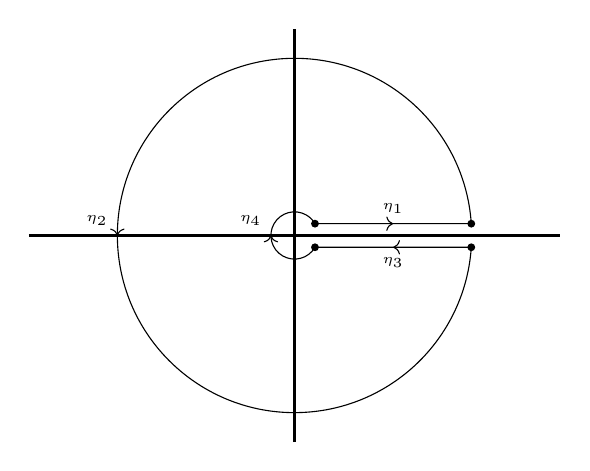
\begin{tikzpicture}[scale=1.5]
          \def\xmin{-2.25} \def\xmax{2.25}
          \def\ymin{-1.75} \def\ymax{1.75}
          \draw[thick] (\xmin,0) -- (\xmax,0);
          \draw[thick] (0,\ymin) -- (0,\ymax);
          
          \draw[->-] ({asin(0.2/2/0.2)}:0.2) -- node[above] {\tiny{\(\eta_{1}\)}} ({asin(0.2/2/1.5)}:1.5);
          \draw[->-] ({asin(0.2/2/1.5)}:1.5) arc ({asin(0.2/2/1.5)}:{360-asin(0.2/2/1.5)}:1.5);
          \node at (-1.5,0) [above left] {\tiny{\(\eta_{2}\)}};
          \draw[->-] ({-asin(0.2/2/1.5)}:1.5) -- node[below] {\tiny{\(\eta_{3}\)}} ({-asin(0.2/2/0.2)}:0.2);
          \draw[->-] ({-asin(0.2/2/0.2)}:0.2) arc ({-asin(0.2/2/0.2)}:{asin(0.2/2/0.2)-360}:0.2);
          \node at (-0.2,0) [above left] {\tiny{\(\eta_{4}\)}};

          \node at ({asin(0.2/2/0.2)}:0.2) [circle,fill,inner sep=1pt]{};
          %\node at ({asin(0.2/2/0.2)}:0.2) [above right] {\tiny{\(\e e^{i\t_{R,\e}}\)}};

          \node at ({asin(0.2/2/1.5)}:1.5) [circle,fill,inner sep=1pt]{};
          %\node at ({asin(0.2/2/1.5)}:1.5) [above right] {\tiny{\(Re^{i\t_{R,\e}}\)}};
          
          \node at ({-asin(0.2/2/0.2)}:0.2) [circle,fill,inner sep=1pt]{};
          %\node at ({-asin(0.2/2/0.2)}:0.2) [below right] {\tiny{\(\e e^{i\left(2\pi-\t_{R,\e}\right)}\)}};

          \node at ({-asin(0.2/2/1.5)}:1.5) [circle,fill,inner sep=1pt]{};
          %\node at ({-asin(0.2/2/1.5)}:1.5) [below right] {\tiny{\(Re^{i(2\pi-\t_{R,\e})}\)}};
        \end{tikzpicture}
        \caption{A keyhole contour.}
        \label{fig:reflection_formula_contour}
      \end{figure}

      Let \(\eta = \sum_{i}\eta_{i}\) be the keyhole contour \cref{fig:reflection_formula_contour} where the large arc has radius \(R\) and the small arc has radius \(\e\). Consider
      \[
        \int_{\eta}\frac{z^{s+1}}{z+1}\,dz.
      \]
      We will evaluate this integral in the limit as \(R \to \infty\) and then as \(\e \to 0\). The contour encloses the only pole of the integrand which is simple at \(z = -1\) and of residue \(e^{\pi i(s-1)}\) (after taking the branch cut \(\log_{0}\) of the logarithm along the positive real axis). So, on the one hand, the residue theorem gives
      \[
        \int_{\eta}\frac{z^{s-1}}{z+1}\,dz = 2\pi ie^{\pi i(s-1)},
      \]
      where in the last equality we have used that \(\log_{0}(-1) = i\pi\) (since this is the branch cut of the logarithm along the positive real axis). On the other hand, the integral is a sum along all four contours. Clearly
      \[
        \lim_{\e \to 0}\lim_{R \to \infty}\int_{\eta_{1}}\frac{z^{s+1}}{z+1}\,dz = \int_{0}^{\infty}\frac{x^{s-1}}{x+1}\,dx.
      \]
      The argument of \(s\) along \(\eta_{3}\) is \(2\pi\) that of it along \(\eta_{1}\). Therefore
      \[
        \lim_{\e \to 0}\lim_{R \to \infty}\int_{\eta_{3}}\frac{z^{s+1}}{z+1}\,dz = e^{2\pi i(s-1)}\int_{0}^{\infty}\frac{x^{s-1}}{x+1}\,dx.
      \]
      The parameterization \(z \mapsto Re^{i\t}\) for \(\eta_{2}\) shows that the integral along this contour tends to zero as \(R \to \infty\). Whence
      \[
        \lim_{\e \to 0}\lim_{R \to \infty}\int_{\eta_{2}}\frac{z^{s+1}}{z+1}\,dz = 0.
      \]
      Similarly, the parameterization \(z \mapsto \e e^{i\t}\) for \(\eta_{4}\) shows that the integral along this contour tends to zero as \(\e \to 0\) and is independent of \(R\). Hence 
      \[
        \lim_{\e \to 0}\lim_{R \to \infty}\int_{\eta_{4}}\frac{z^{s+1}}{z+1}\,dz = 0.
      \]
      All of this shows
      \[
        \lim_{\e \to 0}\lim_{R \to \infty} \int_{\eta}\frac{z^{s-1}}{z+1}\,dz = (1-e^{2\pi i(s-1)})\int_{0}^{\infty}\frac{x^{s-1}}{x+1}\,dx,
      \]
      and together with our previous residue computation gives
      \[
       (1-e^{2\pi i(s-1)})\int_{0}^{\infty}\frac{x^{s-1}}{x+1}\,dx = 2\pi ie^{\pi i(s-1)}.
      \]
      Using the formula \(\sin(\pi s) = \frac{e^{i\pi s}+e^{-i\pi s}}{2i}\), a short computation shows
      \[
        \int_{0}^{\infty}\frac{x^{s-1}}{x+1}\,dx = \frac{\pi}{\sin(\pi s)},
      \]
      as claimed.
    \end{proof}

    It quickly follows from Euler's reflection formula that the gamma function has no zeros. Euler's reflection formula implies
    \[
      \G(s)\G(1-s)\frac{\sin(\pi s)}{\pi} = 1,
    \]
    provided \(s\) is not an integer. Since \(\sin(\pi s)\) is nonzero for such \(s\), \(\G(s)\) is nonzero except possibly at integers. For any positive integer \(\G(s)\) is given by a factorial which is nonzero while for any nonpositive integer \(\G(s)\) has a simple pole. Therefore \(\G(s)\) has no zeros. This implies that the reciprocal of the gamma function is entire. As a nice consequence, we can obtain the meromorphic continuation of the beta function:

    \begin{theorem}\label{thm:continuation_of_beta_function}
      \(B(s,u)\) admits meromorphic continuation to \(\C^{2}\) given by
      \[
        B(s,u) = \frac{\G(s)\G(u)}{\G(s+u)}.
      \]
    \end{theorem}
    \begin{proof}
      As \(\G(s)\) has no zeros, \cref{prop:integral_reprepsentation_for_beta_function} implies
      \[
        B(s,u) = \frac{\G(s)\G(u)}{\G(s+u)},
      \]
      for all \(\s > 0\) and \(\tau > 0\). Then completes the proof since the gamma function admits meromorphic continuation to \(\C\).
    \end{proof}
    
    Now knowing that the gamma function has no zeros, we can use the beta function to prove an important multiplicativity property of the gamma function. This is known as \textit{Legendre's duplication formula}:

    \begin{theorem*}[Legendre's duplication formula]
      For any \(s \in \C-\Z_{\le 0}\), we have
      \[
        \G(s)\G\left(s+\frac{1}{2}\right) = 2^{1-2s}\sqrt{\pi}\G(2s).
      \]
    \end{theorem*}
    \begin{proof}
      By the identity theorem we may assume \(s > 1\). Consider
      \[
        B(s,s) = \int_{0}^{1}x^{s-1}(1-x)^{s-1}\,dx.
      \]
      The change of variables \(x \mapsto \frac{x+1}{2}\) results in
      \[
        2^{1-2s}\int_{-1}^{1}(1-x^{2})^{s-1}\,dx.
      \]
      As the integrand is even, we can express it as
      \[
        2^{2-2s}\int_{0}^{1}(1-x^{2})^{s-1}\,dx.
      \]
      The change of variables \(x \mapsto \sqrt{x}\) yields
      \[
        2^{1-2s}\int_{0}^{1}x^{-\frac{1}{2}}(1-x)^{s-1}\,dx = 2^{1-2s}B\left(\frac{1}{2},s\right).
      \]
      Therefore
      \[
        B(s,s) = 2^{1-2s}B\left(\frac{1}{2},s\right).
      \]
      Invoking \cref{thm:continuation_of_beta_function} to replace the beta functions with gamma functions gives
      \[
        \frac{\G(s)^{2}}{\G(2s)} = 2^{1-2s}\frac{\G\left(\frac{1}{2}\right)\G(s)}{\G\left(s+\frac{1}{2}\right)}.
      \]
      As \(\G(s)\) is nonzero, we may cancel the common \(\G(s)\) factor and use \cref{equ:gamma_function_at_1/2} to obtain
      \[
        \frac{\G(s)}{\G(2s)} = \frac{2^{1-2s}\sqrt{\pi}}{\G\left(s+\frac{1}{2}\right)}.
      \]
      This is equivalent to the desired formula.
    \end{proof}

    As the reciprocal of the gamma function is entire it admits a Hadamard factorization. We will compute this factorization. To this end, recall the limit

    \begin{equation}\label{equ:limit_form_of_exponential}
      \lim_{n \to \infty}\left(\frac{x}{n}+1\right)^{n} = e^{x},
    \end{equation}
    provided \(x > 0\), and that \(\left(\frac{x}{n}+1\right)^{n}\) is monotonically increasing in \(n\). We first prove the following lemma:

    \begin{lemma}\label{lem:Hadamard_factorization_of_gamma_function_lemma}
      For any \(s \in \C-\Z_{\le 0}\), we have
      \[
        \lim_{n \to \infty}\frac{n^{-s}\G(s+n)}{\G(n)} = 1.
      \]
    \end{lemma}
    \begin{proof}
      Apply the functional equation to write
      \[
        \frac{n^{-s}\G(s+n)}{\G(n)} = \left(\frac{s+n-1}{n}\right)\frac{n^{1-s}\G(s-1+n)}{\G(n)},
      \]
      As the limit of the first factor on the right-hand side is \(1\) as \(n \to \infty\), we see that the claim holds for \(s\) if and only if it holds for \(s-1\). Therefore we may assume \(\s < 0\). In other words, it suffices to show
      \[
        \lim_{n \to \infty}\frac{n^{s}\G(n-s)}{\G(n)} = 1,
      \]
      for \(\s > 0\). Appealing to \cref{thm:continuation_of_beta_function}, observe
      \[
       \frac{n^{s}\G(n-s)}{\G(n)} = \frac{n^{s}B(s,n-s)}{\G(s)} = \frac{1}{\G(s)}n^{s}\int_{0}^{\infty}\frac{x^{s-1}}{(x+1)^{n}}\,dx.
      \]
      The change of variables \(x \mapsto \frac{x}{n}\) gives
      \[ 
        \frac{1}{\G(s)}\int_{0}^{\infty}\frac{x^{s-1}}{\left(\frac{x}{n}+1\right)^{n}}\,dx.
      \]
      We now take the limit as \(n \to \infty\). By \cref{equ:limit_form_of_exponential} and that \(\left(\frac{x}{n}+1\right)^{n}\) is monotonically increasing in \(n\), we may employ the monotone convergence theorem to interchange the limit and integral giving
      \[
        \lim_{n \to \infty}\frac{1}{\G(s)}\int_{0}^{\infty}\frac{x^{s-1}}{\left(\frac{x}{n}+1\right)^{n}}\,dx = \frac{1}{\G(s)}\int_{0}^{\infty}e^{-x}x^{s-1}\,dx = 1.
      \]
      This means
      \[
        \lim_{n \to \infty}\frac{n^{s}\G(n-s)}{\G(n)} = 1,
      \]
      as desired.
    \end{proof}

    Obtaining the Hadamard factorization of the reciprocal of the gamma function is now a simple matter. Recall that the Euler-Mascheroni constant \(\g\) is defined as the limit
    \begin{equation}\label{equ:Euler-Mascheroni_constant_definition}
      \g = \lim_{N \to \infty}\left(\sum_{n \le N}\frac{1}{n}-\log(N)\right).
    \end{equation}
    The Hadamard factorization is the following:

    \begin{theorem}\label{thm:Hadamard_factorization_for_reciprocal_of_gamma}
      For any \(s \in \C-\Z_{\le 0}\), we have
      \[
        \frac{1}{\G(s)} = se^{\g s}\prod_{n \ge 1}\left(1+\frac{s}{n}\right)e^{-\frac{s}{n}},
      \]
      where \(\g\) is the Euler-Mascheroni constant.
    \end{theorem}
    \begin{proof}
      Let \(k\) be a positive integer. Apply the functional equation repeatedly to write
      \[
        \frac{1}{\G(s)} = \frac{s(s+1) \cdots (s+k-1)}{\G(s+k)},
      \]
      In view of the identity
      \[
       s+n = e^{\frac{s}{n}}e^{-\frac{s}{n}}n\left(1+\frac{s}{n}\right),
      \]
      we obtain
      \[
        \frac{1}{\G(s)} = se^{\left(1+\frac{1}{2}+\cdots+\frac{1}{k}\right)s}\prod_{1 \le n \le k}\left(1+\frac{s}{n}\right)e^{-\frac{s}{n}}\frac{(k-1)!}{\G(s+k)}.
      \]
      As \(k^{-s}= e^{-s\log(k)}\) and \(\G(k) = (k-1)!\), we may further write
      \[
        \frac{1}{\G(s)} = se^{\left(1+\frac{1}{2}+\cdots+\frac{1}{k}-\log(k)\right)s}\frac{\G(k)}{k^{-s}\G(s+k)}\prod_{1 \le n \le k}\left(1+\frac{s}{n}\right)e^{-\frac{s}{n}}.
      \]
      Taking the limit as \(k \to \infty\), \cref{lem:Hadamard_factorization_of_gamma_function_lemma,equ:Euler-Mascheroni_constant_definition} together imply
      \[
        \frac{1}{\G(s)} = se^{\g s}\prod_{n \ge 1}\left(1+\frac{s}{n}\right)e^{-\frac{s}{n}},
      \]
      as desired.
    \end{proof}   
  \section{Asymptotics}
    Upon inspection of the Hadamard factorization, we find that the reciprocal of the gamma function is of order \(1\). We now turn to analyzing the growth rate of the gamma function itself. In fact, we can obtain a well-known asymptotic formula for the gamma function known as \textit{Stirling's formula}:

    \begin{theorem*}[Stirling's formula]
      Let \(|\arg(s)| < \pi-\e\) and \(|s| > \d\) for some \(\e,\d > 0\). Then
      \[
        \G(s) = \sqrt{2\pi}s^{s-\frac{1}{2}}e^{-s}\left(1+O_{\e,\d}\left(\frac{1}{s}\right)\right).
      \]
      In particular,
      \[
        \G(s) \sim \sqrt{2\pi}s^{s-\frac{1}{2}}e^{-s}.
      \]
    \end{theorem*}
    \begin{proof}
      We begin by additionally assuming \(\s > 0\). Express \(\G(s+1)\) in the complex form
      \[
        \G(s+1) = \int_{0}^{\infty}e^{-z}e^{s\log(z)}\,dz.
      \]
      The change of variables \(z \to s(1+z)\) gives
      \[
        \G(s+1) = s^{s+1}e^{-s}\int_{-1}^{\infty}e^{s(\log(1+z)-z)}\,dz,
      \]
      upon homotoping the transformed contour to \((-1,\infty)\). We will estimate the present integral. Define
      \[
        I(s) = \int_{-1}^{\infty}e^{s(\log(1+z)-z)}\,dz,
      \]
      along with
      \[
        I_{1}(s) = \int_{-1}^{1}e^{s(\log(1+z)-z)}\,dz, \quad \text{and} \quad I_{2}(s) = \int_{1}^{\infty}e^{s(\log(1+z)-z)}\,dz.
      \]
      Then
      \begin{equation}\label{equ:Stirlings_formula_1}
        \G(s+1) = s^{s+1}e^{-s}I(s),
      \end{equation}
      with
      \[
        I(s) = I_{1}(s)+I_{2}(s).
      \]
      Making the change of variables \(z \mapsto 2+z\) to \(I_{2}(s)\) shows
      \[
        I_{2}(s) = e^{-2s}\int_{-1}^{\infty}e^{s(\log(3+z)-z)}\,dz.
      \]
      Since \(\log(3+z) = \log(1+z)+O(1)\), \(I_{2}(s)\) is related to \(I(s)\) via
      \[
        I_{2}(s) = e^{-2s}\int_{-1}^{\infty}e^{s(\log(1+z)-z)}(1+O_{\e,\d}(s))\,dz = I(s)(e^{-2s}+O_{\e,\d}(se^{-2s})).
      \]
      Whence
      \[
        I(s) = I_{1}(s)+I(s)(e^{-2s}+O_{\e,\d}(se^{-2s})).
      \]
      Now isolate \(I(s)\) to see that
      \begin{equation}\label{equ:Stirlings_formula_2}
        I(s) = I_{1}(s)(1+O_{\e,\d}(se^{-2s})).
      \end{equation}
      Therefore it remains to estimate \(I_{1}(s)\). To this end, notice
      \[
        \frac{d}{dz}(\log(1+z)-z) = \frac{1}{1+z}-1 \quad \text{and} \quad \frac{d^{2}}{dz^{2}}(\log(z)-z) = -\frac{1}{(1+z)^{2}}.
      \]
      At \(z = 0\), the first derivative is zero and the second derivative is negative. So taking the Taylor series of \(\log(1+z)-z\) and truncating after the third term gives
      \[
        \log(1+z)-z = -\frac{1}{2}z^{2}+\frac{1}{3}z^{3}+O(z^{4}).
      \]
      Use this estimate in \(I_{1}(s)\) to write
      \[
        I_{1}(s) = \int_{-1}^{1}e^{-\frac{s}{2}z^{2}}e^{\frac{1}{3}sz^{3}+O_{\e,\d}(sz^{4})}\,dz.
      \]
       Considering the Taylor series of \(e^{z}\) and truncating after the second term, we find that
      \[
        e^{\frac{1}{3}sz^{3}+O_{\e,\d}(sz^{4})} = 1+\frac{1}{3}sz^{3}+O_{\e,\d}(sz^{4})+O_{\e,\d}(s^{2}z^{6}).
      \]
      Plugging this estimate into the previous integral yields
      \[
        I_{1}(s) = \int_{-1}^{1}e^{-\frac{s}{2}z^{2}}\left(1+\frac{1}{3}sz^{3}+O_{\e,\d}(sz^{4})+O_{\e,\d}(s^{2}z^{6})\right)\,dz.
      \]
      Since the first and second terms in the asymptotic are even and odd in \(z\) respectively, symmetry forces
      \[
        I_{1}(s) = 2\int_{0}^{1}e^{-\frac{s}{2}z^{2}}\left(1+O_{\e,\d}(sz^{4})+O_{\e,\d}(s^{2}z^{6})\right)\,dz.
      \]
      Performing the change of variables \(z \mapsto \sqrt{\frac{2z}{s}}\), and noting that \(z\) is bounded (so that the \(O\)-estimates are independent of \(z\)), results in
      \begin{equation}\label{equ:Stirlings_formula_3}
        I_{1}(s) = \sqrt{2}s^{-\frac{1}{2}}\int_{0}^{\frac{|s|}{2}}e^{-z}z^{-\frac{1}{2}}\,dz\left(1+O_{\e,\d}\left(\frac{1}{s}\right)\right),
      \end{equation}
      where we have homotoped the transformed contour to \(\left(0,\frac{|s|}{2}\right)\). We will further estimate the remaining integral. Observe that
      \[
        \int_{0}^{\frac{|s|}{2}}e^{-z}z^{-\frac{1}{2}}\,dz = \G\left(\frac{1}{2}\right)-\int_{\frac{|s|}{2}}^{\infty}e^{-z}z^{-\frac{1}{2}}\,dz = \sqrt{\pi}-\int_{\frac{|s|}{2}}^{\infty}e^{-z}z^{-\frac{1}{2}}\,dz,
      \]
      where we have used \cref{equ:gamma_function_at_1/2} to evaluate the gamma function. By the exponential decay of the integrand, we have say
      \[
        \int_{\frac{|s|}{2}}^{\infty}e^{-z}z^{-\frac{1}{2}}\,dz = O_{\e,\d}\left(\int_{\frac{|s|}{2}}^{\infty}\frac{1}{z^{3}}\,dz\right) = O_{\e,\d}\left(\frac{1}{s^{2}}\right),
      \]
      so that 
      \begin{equation}\label{equ:Stirlings_formula_4}
        \int_{0}^{\frac{|s|}{2}}e^{-z}z^{-\frac{1}{2}}\,dz = \sqrt{\pi}+O_{\e,\d}\left(\frac{1}{s^{2}}\right).
      \end{equation}
      Substituting \cref{equ:Stirlings_formula_4} into \cref{equ:Stirlings_formula_3} gives
      \begin{equation}\label{equ:Stirlings_formula_5}
        I_{1}(s) = \sqrt{2\pi}s^{-\frac{1}{2}}\left(1+O_{\e,\d}\left(\frac{1}{s}\right)\right).
      \end{equation}
      Combining \cref{equ:Stirlings_formula_1,equ:Stirlings_formula_2,equ:Stirlings_formula_5} yields
      \[
        \G(s+1) = \sqrt{2\pi}s^{s+\frac{1}{2}}e^{-s}\left(1+O_{\e,\d}\left(\frac{1}{s}\right)\right).
      \]
      Using the functional equation gives
      \[
        \G(s) = \sqrt{2\pi}s^{s-\frac{1}{2}}e^{-s}\left(1+O_{\e,\d}\left(\frac{1}{s}\right)\right).
      \]
      This proves the asymptotic formula when \(\s > 0\). In fact, applying the functional equation repeatedly shows
      \[
        \G(s-n) = \sqrt{2\pi}\frac{s^{s-\frac{1}{2}}}{(s-1)(s-2) \ldots (s-n)}e^{-s}\left(1+O_{\e,\d}\left(\frac{1}{s}\right)\right),
      \]
      for any nonnegative integer \(n\). As \(\frac{1}{s-k} = \frac{1}{s}+O_{\e,\d}\left(\frac{1}{s^{2}}\right)\), it follows that
      \[
        \G(s-n) = \sqrt{2\pi}s^{s-n-\frac{1}{2}}e^{-s}\left(1+O_{\e,\d}\left(\frac{1}{s}\right)\right).
      \]
      Since \(n\) was arbitrary, this proves the asymptotic formula when \(\s \le 0\) as well. The asymptotic equivalence follows immediately since it is a strictly weaker asymptotic.
    \end{proof}

    We now turn to estimates for the gamma function in vertical strips. The first of which is useful asymptotic equivalence showing that the gamma function admits exponential decay.
    
    \begin{corollary}\label{equ:weaker_Stirling_formula_1}
      Let \(|\arg(s)| < \pi-\e\) and \(|s| > \d\) for some \(\e,\d > 0\) and suppose \(\s\) is bounded. Then
      \[
        \G(s) \sim \sqrt{2\pi}|t|^{\s-\frac{1}{2}}e^{-\frac{\pi}{2}|t|}.
      \]
    \end{corollary}
    \begin{proof}
      Stirling's formula implies
      \[
        \G(s) \sim \sqrt{2\pi}e^{\left(s-\frac{1}{2}\right)\log(s)}e^{-s}.
      \]
      Writing \(\log(s) = \log|s|+i\arg(s)\), this asymptotic becomes
      \[
        \G(s) \sim \sqrt{2\pi}e^{\left(s-\frac{1}{2}\right)\log|s|}e^{\left(s-\frac{1}{2}\right)i\arg(s)}e^{-s}.
      \]
      Taking absolute values further implies
      \[
        \G(s) \sim \sqrt{2\pi}e^{\left(\s-\frac{1}{2}\right)\log|s|}e^{-(t\arg(s)+\s)}.
      \]
      As \(\s\) is bounded, we have the asymptotics \(|s| = |t|+o(1)\) and \(\arg(s) = \sgn(t)\frac{\pi}{2}+o(1)\). These estimates along with the fact \(-t\sgn(t) = -|t|\) together imply
      \[
        \G(s) \sim \sqrt{2\pi}e^{\left(\s-\frac{1}{2}\right)\log|t|}e^{-\frac{\pi}{2}|t|}.
      \]
      This is equivalent to the desired asymptotic.
    \end{proof}

    We can use \cref{equ:weaker_Stirling_formula_1} to obtain weaker estimates valid on the negative real axis away from the poles of the gamma function.

    \begin{corollary}\label{equ:weaker_Stirling_formula_2}
      Suppose \(\s\) is bounded. Then
      \[
        \G(s) \ll_{\e} (|t|+3)^{\s-\frac{1}{2}}e^{-\frac{\pi}{2}|t|} \quad \text{and} \quad \frac{1}{\G(s)} \ll (|t|+3)^{\frac{1}{2}-\s}e^{\frac{\pi}{2}|t|},
      \]
      where in the former estimate we assume \(s\) is at least distance \(\e\) away from the poles of the gamma function in this vertical strip.
    \end{corollary}
    \begin{proof}
      Let \(s\) be in the given region and assume \(|t| > \e\). \cref{equ:weaker_Stirling_formula_1} implies the strictly weaker estimates
      \[
        \G(s) \ll_{\e} |t|^{\s-\frac{1}{2}}e^{-\frac{\pi}{2}|t|} \quad \text{and} \quad \frac{1}{\G(s)} \ll_{\e} |t|^{\frac{1}{2}-\s}e^{\frac{\pi}{2}|t|}.
      \]
      Since the gamma function is holomorphic and bounded on the compact set defined by \(\s\) being bounded and \(|t| \le \e\) with \(s\) at least distance \(\e\) away from its poles, we may relax the condition \(|t| \ge 1\) provided we replace \(|t|\) with \(|t|+3\). This proves the first estimate. The second estimate follows by an analogous argument but holds in the entire vertical strip as the reciprocal of the gamma function is entire.
    \end{proof}

    The choice of \(3\) in \(|t|+3\) in \cref{equ:weaker_Stirling_formula_2} is a matter of convenience as we could use any large positive constant. In particular, it is useful when taking logarithms as \(\log(|t|+3) \ge 1\).

    Having discussed the major properties of the gamma function, we now introduce a related function. We call \(\frac{\G'}{\G}(s)\) the \textit{digamma function}. In other words, the digamma function is the logarithmic derivative of the gamma function. From \cref{thm:continuation_of_gamma_function}, it is meromorphic on \(\C\) with simple poles at the nonpositive integers whose residues are all \(-1\). Taking the logarithmic derivative of the functional equation shows
    \[
      \frac{\G'}{\G}(s+1) = \frac{\G'}{\G}(s)+\frac{1}{s}.
    \]
    In similar spirit, we may take the logarithmic derivative of the Hadamard factorization of the reciprocal of the gamma function to obtain a summation formula for the digamma function.

    \begin{corollary}\label{cor:logarithmic_derivative_of_gamma}
      For all \(s \in \C-\Z_{\le 0}\), we have
      \[
        \frac{\G'}{\G}(s+1) = -\g+\sum_{n \ge 1}\left(\frac{1}{n}-\frac{1}{s+n}\right),
      \]
      where \(\g\) is the Euler-Mascheroni constant.
    \end{corollary}
    \begin{proof}
      As the gamma function has no zeros, we may use the functional equation to write
      \[
        \frac{1}{\G(s+1)} = \frac{1}{s\G(s)}.
      \]
      Taking the logarithmic derivative by using the Hadamard factorization shows
      \[
        -\frac{\G'}{\G}(s+1) = \g+\sum_{n \ge 1}\left(\frac{1}{s+n}-\frac{1}{n}\right).
      \]
      This is equivalent to the desired formula.
    \end{proof}
    
    As for estimates involving the digamma function, we can appeal to Stirling's formula to obtain as asymptotic formula.

    \begin{proposition}\label{equ:approximtion_for_digamma}
      Let \(|\arg(s)| < \pi-\e\) and \(|s| > \d\) for some \(\e,\d > 0\). Then
      \[
        \frac{\G'}{\G}(s) = \log(s)+O_{\e,\d}\left(\frac{1}{s}\right).
      \]
      In particular,
      \[
        \frac{\G'}{\G}(s) \sim \log(s).
      \]
    \end{proposition}
    \begin{proof}
      Taking the logarithm of Stirling's formula gives
      \[
        \log\G(s) = \frac{1}{2}\log(2\pi)+\left(s-\frac{1}{2}\right)\log(s)-s+O_{\e,\d}\left(\frac{1}{s}\right),
      \]
      Set \(g(s) = \frac{1}{2}\log(2\pi)+\left(s-\frac{1}{2}\right)\log(s)-s\). Then we may write
      \[
        \log\G(s)-g(s) = O_{\e,\d}\left(\frac{1}{s}\right).
      \]
      Now write
      \[
        \log\G(s) = g(s)+\log\G(s)-g(s),
      \]
      and note that \(g'(s) = \log(s)-\frac{1}{2s}\). Taking the derivative of this identity and using Cauchy's integral formula to express the derivative of \(\log\G(s)-g(s)\), we obtain
      \[
        \frac{\G'}{\G}(s) = \log(s)-\frac{1}{2s}+\frac{1}{2\pi i}\int_{\eta}\frac{\log\G(u)-g(u)}{(u-s)^{2}}\,du,
      \]
      where \(\eta\) is a circle about \(s\) of sufficiently small radius \(r\) depending upon \(\e\) and \(\d\). The parameterization \(u \mapsto s+re^{i\t}\) for \(\eta\) shows that
      \[
        \frac{1}{2\pi i}\int_{\eta}\frac{\log\G(u)-g(u)}{(u-s)^{2}}\,du = O_{\e,\d}\left(\frac{1}{s}\right),
      \]
      in view of our estimate for \(\log\G(s)-g(s)\). Whence
      \[
        \frac{\G'}{\G}(s) = \log(s)+O_{\e,\d}\left(\frac{1}{s}\right).
      \]
      This proves the asymptotic formula. The asymptotic equivalence is immediate as it is a strictly weaker asymptotic.
    \end{proof}

    Just as for the gamma function, it is possible to obtain estimates for the digamma function in vertical strips.

    \begin{corollary}\label{equ:weaker_approximtion_for_digamma_1}
      Let \(|\arg(s)| < \pi-\e\) and \(|s| > \d\) for some \(\e,\d > 0\) and suppose \(\s\) is bounded. Then
      \[
        \frac{\G'}{\G}(s) \sim \log|s|.
      \]
    \end{corollary}
    \begin{proof}
      Writing \(\log(s) = \log|s|+i\arg(s)\), \cref{equ:approximtion_for_digamma} gives
      \[
        \frac{\G'}{\G}(s) \sim (\log|s|+i\arg(s)).
      \]
      As \(\s\) is bounded, we have \(\arg(s) = O(1)\). This asymptotic implies
      \[
        \frac{\G'}{\G}(s) \sim \log|s|,
      \]
      as desired.
    \end{proof}

    We can use \cref{equ:weaker_approximtion_for_digamma_1} to obtain a weaker estimate valid on the negative real axis away from the poles of the gamma function.

    \begin{corollary}\label{equ:weaker_approximtion_for_digamma_2}
      Suppose \(\s\) is bounded and \(s\) is at least distance \(\e\) away from the poles of the gamma function in this vertical strip. Then
      \[
        \frac{\G'}{\G}(s) \ll_{\e} \log(|s|+3).
      \]
    \end{corollary}
    \begin{proof}
      Let \(s\) be in the given region and assume \(|t| > \e\). \cref{equ:weaker_approximtion_for_digamma_1} implies the strictly weaker estimate
      \[
        \frac{\G'}{\G}(s) \ll_{\e} \log|s|.
      \]
      Since the digamma function is holomorphic and bounded on the compact set defined by \(\s\) being bounded and \(|t| \le \e\) with \(s\) at least distance \(\e\) away from its poles, we may relax the condition \(|t| \ge 1\) provided we replace \(|s|\) with \(|s|+3\). The estimate follows.
    \end{proof}

    The choice of \(3\) in \(|s|+3\) at the end of \cref{equ:weaker_approximtion_for_digamma_2} is a matter of convenience as could use any large positive constant. In particular, it is useful when taking logarithms as \(\log(|s|+3) \ge 1\).
\end{document}